\documentclass[10pt]{article}
\usepackage{icmlko}

\icmlmeta{IP 파운데이션 월드모델}{83}{둘째 출처가 나머지 여섯보다 값졌다}{도메인은 정확도가 아니라 정밀도를 산다 --- 그리고 노트 81의 신뢰도 하나를 철회한다}

\begin{document}

\twocolumn[
\icmlheader

\begin{abstract}
먼저 철회할 것이 있다. 노트 81이 애니 라벨 신뢰도를 $+$0.784(32건)로 적고
``웹툰$\leftrightarrow$만화의 $+$0.524와 겹치지 않으니 두 쌍의 신뢰도가 실제로
다르다''고 했다. \textbf{매칭을 32건에서 87건으로 늘리니 $+$0.5554}
{[}$+$0.336, $+$0.734{]}\textbf{로 내려온다.} 원래 32건은 제목이 정확히 맞는
것만 걸린 유명작 편향이었다. \textbf{두 쌍이 0.52와 0.56으로 겹치고, 천장
추정은 0.72$\sim$0.75로 좁혀진다.} 본론은 노트 82가 남긴 질문이다 --- 출처
하나를 빼는 것이 무해하다면 몇 개까지 빼도 되나. 대상 집합을 고정하고 출처를
$m$개만 써서 앙상블했다. \textbf{곡선이 $m=2$에서 이미 평평하다} ---
$m{=}1\to2$가 $+$0.0139인데 $m{=}2\to8$이 다 합쳐 $+$0.0099다. \textbf{둘째
출처가 나머지 여섯을 합친 것보다 값지다.} 적합이 $\rho(m)=0.383+0.0109\ln m$이라
출처를 스물로 늘려도 $+$0.4157, 서른으로 늘려도 $+$0.4201이다(지금 여덟이
$+$0.4030). \textbf{도메인을 더 모으는 것은 정확도를 거의 안 산다.} 그런데
노트 81에서 열째 도메인이 반폭을 0.0388에서 0.0334로 줄였다. \textbf{도메인은
정확도가 아니라 정밀도를 산다.} 그러면 정확도의 남은 지렛대는 하나뿐이다 ---
배선은 닫혔고(노트 76) 부분집합도 닫혔고(노트 80) 도메인도 닫혔으니
\textbf{새 물리량}이다.
\end{abstract}
]

\begin{figure*}[t]
\centering
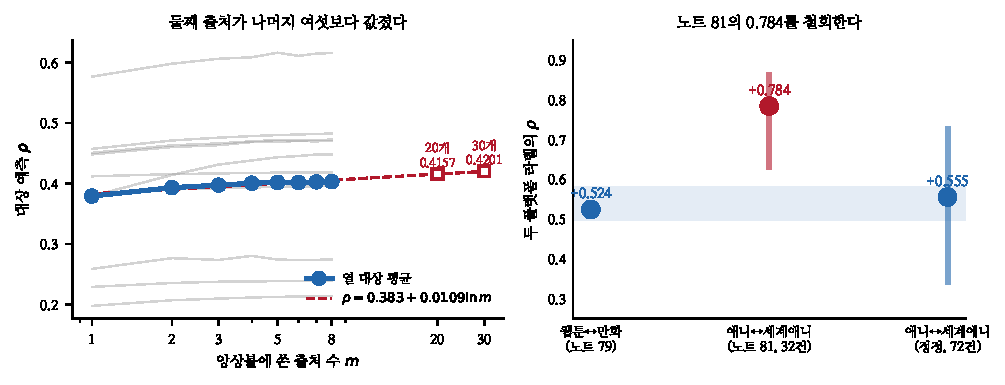
\includegraphics[width=\textwidth]{figs/hm.pdf}
\caption{왼쪽 --- 출처 $m$개로 앙상블할 때(회색이 대상별). 오른쪽 --- 라벨
신뢰도 두 쌍과 정정.}
\end{figure*}

\section{철회 --- 애니 신뢰도 0.784}

\begin{table}[t]
\centering\tsize
\caption{같은 작품을 두 플랫폼이 잰 값의 상관.}
\begin{tabular}{lrrl}
\toprule
쌍 & $n$ & $\rho$ & 95\% 구간 \\
\midrule
웹툰 $\leftrightarrow$ 만화(노트 79) & 327 & $+$0.524 & --- \\
애니 $\leftrightarrow$ 세계애니(노트 81) & 32 & $+$0.784 & $[+0.625, +0.870]$ \\
\textbf{애니 $\leftrightarrow$ 세계애니(정정)} & \textbf{72} & \textbf{$+$0.555} &
$[+0.336, +0.734]$ \\
\bottomrule
\end{tabular}
\end{table}

노트 81의 32건은 라프텔 한국어 제목이 AniList 제목과 \emph{정확히} 맞는 것만
걸린 것이라 유명작에 쏠려 있었다. AniList 검색 API로 라프텔 제목 2,073개를
직접 조회해 87건(중복 제거 72건)으로 늘리니 $+$0.5554로 내려온다.

\claimx{노트 81의 ``두 쌍의 신뢰도가 실제로 다르다''를 철회한다. 두 쌍이
$+$0.524와 $+$0.555로 겹치고, 라벨 신뢰도는 \textbf{0.52$\sim$0.56}, 천장은
\textbf{0.72$\sim$0.75}로 좁혀진다.}{정정한 72건에는 시즌 오매칭이 섞여 있다
(AniList 검색이 ``진격의 거인''에 최종 시즌을 준다). 그 잡음이 $\rho$를 낮추므로
진값은 0.555보다 높을 것이다.}

천장이 0.72$\sim$0.75면 현재 위치는 --- 팝업 제품 수치 $+$0.527이 71\%,
판정치 $+$0.404가 55\%다.

\section{출처는 둘이면 거의 다 온다}

\begin{table}[t]
\centering\tsize
\caption{출처 $m$개로 앙상블. 열 대상 평균, 조합마다 60회 표집.}
\begin{tabular}{rrr}
\toprule
$m$ & 평균 $\rho$ & 직전 대비 \\
\midrule
1 & $+$0.3792 & --- \\
\textbf{2} & \textbf{$+$0.3931} & \textbf{$+$0.0139} \\
3 & $+$0.3973 & $+$0.0042 \\
4 & $+$0.4004 & $+$0.0031 \\
5 & $+$0.4019 & $+$0.0015 \\
6 & $+$0.4017 & $-$0.0002 \\
7 & $+$0.4027 & $+$0.0010 \\
8 & $+$0.4030 & $+$0.0003 \\
\bottomrule
\end{tabular}
\end{table}

\claimx{앙상블은 출처 두 개에서 이미 포화한다. $m{=}1\to2$가 $+$0.0139이고
$m{=}2\to8$이 여섯 개를 더해 $+$0.0099다 --- \textbf{둘째 출처가 나머지 여섯을
합친 것보다 값지다.}}{조합을 무작위로 뽑아 평균했으므로 ``어떤 둘이냐''는 안
봤다. 좋은 둘을 고르면 더 높고 나쁜 둘은 더 낮을 것이며, 고르려면 대상 라벨이
든다(노트 71).}

\begin{table}[t]
\centering\tsize
\caption{$\rho(m)=0.3829+0.0109\ln m$ 의 외삽.}
\begin{tabular}{rr}
\toprule
출처 수 & 예상 $\rho$ \\
\midrule
8 (지금) & $+$0.4030 \\
12 & $+$0.4101 \\
20 & $+$0.4157 \\
30 & $+$0.4201 \\
\bottomrule
\end{tabular}
\end{table}

도메인을 지금의 세 배로 늘려도 $+$0.017이다. \textbf{정확도를 사려면 도메인이
아니다.}

\section{도메인은 정밀도를 산다}

\begin{table}[t]
\centering\tsize
\caption{도메인을 하나 더할 때 무엇이 바뀌나.}
\begin{tabular}{lrr}
\toprule
& 9도메인 & 10도메인 \\
\midrule
판정치 & $+$0.4003 & $+$0.4038 \\
\textbf{구간 반폭} & 0.0388 & \textbf{0.0334} \\
\bottomrule
\end{tabular}
\end{table}

노트 81의 짝지은 측정이다. 평균은 $+$0.0035 오르는데 반폭은 14\% 줄었다.
\textbf{도메인의 값은 정밀도에 있다.}

\begin{quote}\fontsize{9.5}{11.5}\selectfont
둘을 나눠 보면 로드맵이 정리된다. \textbf{구간을 좁히려면 도메인}(노트 69의
셀 수 법칙, 다섯에서 열까지 유지). \textbf{평균을 올리려면 도메인이 아니다}
--- 배선은 닫혔고(노트 76) 부분집합도 닫혔고(노트 80) 도메인도 닫혔다.
남은 것은 \textbf{새 물리량}이다.
\end{quote}

\section{남은 지렛대}

\begin{table}[t]
\centering\tsize
\caption{지렛대 점검표.}
\begin{tabular}{ll}
\toprule
배선 재탐색 & 닫힘(노트 76, 후보 92개 전부 문턱 아래) \\
잡음 부분집합 & 닫힘(노트 80, 45개 중 채택 0) \\
도메인 추가 & 정밀도만(이 노트) \\
도메인 제거 & 무의미(노트 82, 전부 보류) \\
방향 교정 & 무의미(노트 73 · 82의 희석) \\
학습된 가중치 & 무의미(노트 73, 게이트가 균등과 같음) \\
레코드 추가 & 포화(노트 68) \\
\textbf{새 물리량} & \textbf{미탐색} \\
\bottomrule
\end{tabular}
\end{table}

노트 76이 배선을 닫으며 반증 조건을 이렇게 적었다 --- ``후보 풀이 내가 등록한
것뿐이다. \textbf{새 물리량을 수집해 후보에 넣으면 다를 수 있다}.'' 그것이
지금 유일하게 안 열어 본 문이다.

\section{한계}

\begin{itemize}[leftmargin=1.1em,itemsep=0.15em]
\item 학습 곡선을 무작위 조합으로 냈다. 실제로는 출처를 고를 수 있으므로
      상한이 더 높다 --- 다만 고르려면 대상 라벨이 든다.
\item $\ln m$ 적합은 여덟 점이다. 스물 · 서른의 외삽은 가정이다.
\item 정정한 애니 신뢰도 72건에 시즌 오매칭이 섞여 있어 아래로 편향됐다.
\item ``새 물리량이 유일한 지렛대''는 지금까지 시도한 것들의 목록에서 나온
      말이다. 안 떠올린 것이 있을 수 있다.
\item 곡선을 판정치(대상 평균)로 냈다. 팝업만 보면 다를 수 있는데 노트 75가
      팝업으로는 못 잰다고 했다.
\end{itemize}

\section{다음}

\begin{enumerate}[leftmargin=1.3em,itemsep=0.15em]
\item \textbf{새 물리량을 수집한다.} 기존 도메인에 지금 없는 축 재료를 붙인다
      --- 예를 들어 가격대별 판매 구성, 리뷰 텍스트 길이, 출시 시기의 경쟁 밀도.
\item 좋은 출처 둘을 고르는 값 --- 대상 라벨 $k$건으로 상위 둘을 고르면
      무작위 둘보다 얼마나 나은가.
\item 팝업 라벨의 신뢰도. 천장이 0.72$\sim$0.75인지 팝업에서도 그런지.
\item 열한째 도메인은 \emph{정밀도}가 필요할 때만.
\end{enumerate}

\vspace{0.6em}
\hrule height 0.3pt
\vspace{0.5em}
{\footnotesize
\textbf{참고문헌}\\[0.3em]
Breiman, L. (1996). Bagging predictors. \emph{Machine Learning}, 24(2), 123--140.\\[0.15em]
Kuncheva, L. I., Whitaker, C. J. (2003). Measures of diversity in classifier
ensembles. \emph{Machine Learning}, 51(2), 181--207.\\[0.15em]
Lord, F. M., Novick, M. R. (1968). \emph{Statistical Theories of Mental Test
Scores}. Addison-Wesley.\\[0.15em]
Ben-David, S. et al. (2010). A theory of learning from different domains.
\emph{Machine Learning}, 79(1--2), 151--175.\\[0.15em]
Efron, B., Tibshirani, R. J. (1993). \emph{An Introduction to the Bootstrap}.
Chapman \& Hall.
}

\end{document}
